% !TeX root = ../tut10.tex
% !TeX encoding = latin1

\section[Effizienz]{Algorithmen-Effizienz}
\subsection*{}
\begin{frame}
			\frametitle{Aufwandsklassen}
			\begin{block}{Fallunterscheidung: Aufwandsklassen}
                \begin{description}
                    \item[$O$-Kalkül] Obere Schranke, die der Algorithmus erreichen, aber nicht überschreiten kann
                    \item[$\Omega$-Kalkül] Untere Schranke und ein "'Mindestaufwand"', den der Algorithmus hat
					\item[$\Theta$-Kalkül] Schnittmenge der Betrachtung aus $\Omega(n)$ und
					$O(n)$.\\ Es entsteht eine Art "`Korridor"', den der Algorithmus nie
					verlässt.
                \end{description}
			\end{block}
\end{frame}

\subsection*{}
\begin{frame}
  \frametitle{$O$-Kalkül}
    \begin{block}{Definition}
          $O(g(n))=\{f(n)| \exists c > 0 \ \exists n_{0} \in \mathbb{N}\ \forall n \ge n_{0}: 0 \le f(n) \le c\cdot g(n)\}$
    \end{block}

    \begin{block}{Umgangssprachlich}
        $O(g(n))$ enthält alle nicht-negativen Funktionen, die höchstens so schnell wie $g(n)$ wachsen.

        Dabei kümmern wir uns nicht

  \begin{itemize}
    \item darum, was am Anfang passiert ($\exists n_0\in\mathbb{N}$ \ldots $\forall n\ge n_0$).
    \item um einfache Faktoren ($\exists c\in\mathbb{R}$ \ldots $c\cdot g(n)$).
  \end{itemize}
  \end{block}
\end{frame}

\begin{frame}
			\frametitle{Aufwandsklassen}
		\only<1>{
				Obere asymptotische Schranke\\
				$O(g(n)) = \{f(n) \,|$\\$ \exists c \in \mathbb{R}^+, n_0 \in \mathbb{N} \,\forall n > n_0 : 0 \leq f (n) \leq c \cdot g(n)\}$\\
\vspace{3ex}
				Untere asymptotische Schranke\\
				$\Omega(g(n)) = \{f (n) \,|$\\$ \exists c \in \mathbb{R}^+, n_0 \in \mathbb{N} \,\forall n > n_0 : 0 \leq c \cdot g(n) \leq f (n)\}$\\
\vspace{3ex}
				Asymptotisch scharfe Schranke\\
				$\Theta(g(n)) = \{f (n) \,|$\\$ \exists c_1, c_2 \in \mathbb{R}^+, n_0 \in \mathbb{N} \,\forall n > n_0 :
					0 \leq c_1 \cdot g(n) \leq f (n) \leq c_2 \cdot g(n)\}$\\
		}
		\begin{block}{\bf Beachte:}
		Alle Kalküle geben eine {\bf Menge} von Funktionen an. $f(n) = O(n^2)$ bedeutet also eigentlich $f(n) \in O(n^2)$!
		\end{block}
\end{frame}


\begin{frame}
			\frametitle{Rechenregeln}
			\begin{block}{Reflexivität}
                \begin{itemize}
                    \item $f(n) \in O(f(n))$
                    \item $g(n) \in \Omega(g(n))$
					\item $h(n) \in \Theta(h(n))$
                \end{itemize}
			\end{block}
			\begin{block}{Symmetrie}
					Hier gilt nur:  $f(n) \in \Theta(g(n)) \Leftrightarrow g(n) \in \Theta(f(n))$
			\end{block}
			\begin{block}{asymptotisches Wachstum}
				\begin{itemize}
                    \item $O(n^2 + n + log(n)) = O(n^2)$
                    \item $\Omega(n^2 + n + log(n)) = \Omega(n^2) \subset \Omega(log(n))$
                \end{itemize}
			\end{block}
\end{frame}

\begin{frame}
			\frametitle{Beispiel}
		\begin{block}{\bf Es gilt nicht:}
		$f(n) \not\in \Theta(g(n)) \Rightarrow g(n) \in O(f(n)) \vee f(n) \in O(g(n))$
		\end{block}

		\begin{block}{\bf Sucht Gegenbeispiele:}
		\begin{itemize}\pause
			\item $|\cos(n)| * n$ und \pause $n$
			\item $n$ und \pause $f(n)=$ $n$ für gerade, $0$ für ungerade Werte von $n$
		\end{itemize}
		\end{block}
\end{frame}



\section{Endliche Automaten} %%%%%%%%%%%%%%%%%%%%%%%%%%%%%% Endliche Automaten %%%%%%%%%%%%%%%%%%%%
\subsection*{}
\begin{frame}
  \frametitle{Endlich ein Automat!}

  \begin{block}{Wozu?}
    Ein endlicher Automat ist gerade mächtig genug, um einen regulären Ausdruck zu erkennen. Der Vorteil von endlichen Automaten ist, dass sie sehr einfach zu implementieren sind.
  \end{block}
  \pause
  \begin{block}{Was braucht man?}
    \begin{itemize}
      \item endliche Menge $Z$ von Zuständen
      \item ein Anfangszustand $z_0 \in Z$
      \item ein Eingabealphabet $X$
      \item Zustandsübergangsfunktion $f:Z \times X \rightarrow Z$
      \item ein Ausgabealphabet $Y$
      \item eine Ausgabefunktion (abhängig vom Typ des Automaten)
    \end{itemize}
  \end{block}
\end{frame}

\begin{frame}
  \frametitle{Endlich ein Automat!}

  \begin{block}{Wie arbeitet er?}
    Das Lesen eines Zeichens $x \in X$ führt zu einem Zustandsübergang vom
    aktuellen Zustand $z \in Z$ in einen neuen Zustand $z' \in Z$
    \begin{itemize}
      \item Notation: $f(z,x)=z'$
      %    \item Bei gegebenem $q$ bestimmt $a$ den Nachfolgerzustand bzw. bei
      %      gegebenem $a$ hängt die Wirkung $q'$ vom bisherigen Zustand $q$ ab
      \item Der Zustand läßt sich als ein \textbf{Gedächtnis} über die
        Vorgeschichte, also die bisher eingegebenen Zeichen, auffassen.\\
        Dieses ist leider nur \textbf{endlich} (endliche Menge an Zuständen!)
    \end{itemize}
  \end{block}
\end{frame}

\begin{frame}
  \frametitle{Darstellung von endlichen Automaten als Graphen}

  \begin{columns}
  \column{.5\textwidth}
    \textbf{Zustandsmenge} $Z = \{z_0, z_1, \ldots, z_n\}$ des endlichen Automaten
      lassen sich als Ecken eines Graphen auffassen
  \column{.4\textwidth}
    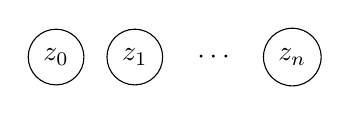
\begin{tikzpicture}
      \node[draw,circle] at (0,0) {$z_0$};
      \node[draw,circle] at (1,0) {$z_1$};
      \node              at (2,0) {$\cdots$};
      \node[draw,circle] at (3,0) {$z_n$};
    \end{tikzpicture}\\
  \end{columns}
  \pause
  \vspace{2em}

  \begin{columns}
  \column{.5\textwidth}
    \textbf{Zustandsübergänge} $f(z_i,x)=z_j$ mit $x \in X$ entsprechen
      markierten gerichteten Kanten
  \column{.4\textwidth}
    \begin{tikzpicture}
      \node[draw,circle] (qi) at (0,0) {$z_i$};
      \node[draw,circle] (qj) at (2,0) {$z_j$};
      \path[draw,-fat] (qi) -- (qj) node[midway,above] {$x$};
    \end{tikzpicture}
  \end{columns}
  \pause
  \vspace{2em}

  Ein im endlichen Automaten erreichter Zustand $z_k$ ist durch den
  Anfangszustand $z_0$ und die bisher eingegebene Zeichenreihe $w \in X^*$ mit
  $w = x_1\ldots x_i$ bestimmt \\
%  \\ Die Graph-Notation ist hierbei: $q_0\Rightarrow^{+}q_k$ bzw.
%  $q_0\Rightarrow^{*}q_k$
\end{frame}

\begin{frame}
	\frametitle{$f^*$ und $f^{**}$}

	\begin{block}{$f^*$}
	   Nach Eingabe des ganzen Wortes $w \in X^*$ erreichen wir den Zustand $f^*: Z \times X^* \rightarrow Z $ mit
      \begin{align*}
				  f^*(z, \epsilon) &= z \\
				  \forall w\in X^*: \forall x\in X: \text{\quad}
				  f^*&(z, wx)   = f(f^*(z,w),x)
			\end{align*}
	\end{block}
	\pause
	\begin{block}{$f^{**}$}
		   Nach Eingabe des ganzen Wortes $w \in X^*$ haben wir die Zustände $f^{**}: Z \times X^* \rightarrow Z^* $ durchlaufen, mit
			\begin{align*}
				  f^{**}(z, \epsilon) &= z \\
				  \forall w\in X^*:  x\in X: \text{\qquad}
				  f^{**}(z, wx&)   = f^{**}(z,w) f(f^*(z,w),x)
			\end{align*}
	\end{block}
%  Beide Definitionen lassen sich auch alternativ definieren, indem man nicht, das letzte Symbol des Eingabewortes zuerst betrachtet, sondern das erste.
\end{frame}

\begin{frame}
	\frametitle{Ein Beispielautomat...}
		\begin{figure}
			\centering
				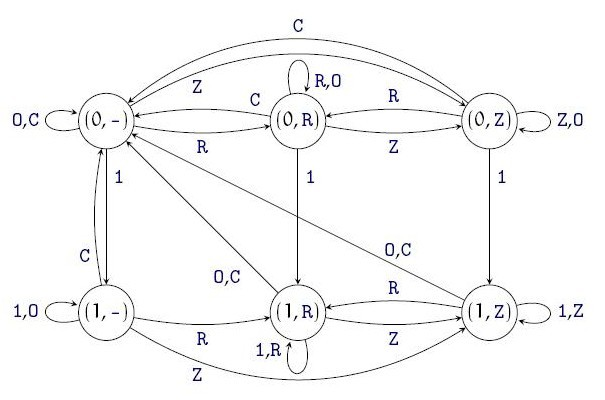
\includegraphics[height=5.7cm]{src/tut10_automat1.jpg}
		\end{figure}
		Was ist $f^*((0,-),R10)$? Was ist $f^{**}((0,-),R10)$?
\end{frame}

\begin{frame}
  \frametitle{Arten von Automaten}

  Es gibt zwei Arten, wie ein Automat eine Ausgabe tätigen kann. Wir unterscheiden dabei:
  \pause
  \begin{block}{Mealy-Automat}
    \begin{itemize}
      \item Erzeugung einer Ausgabe bei jedem Zustandsübergang
      \item Ausgabefunktion $g: Z \times X \rightarrow Y^*$
      \item Markieren der Kanten mit $x_i|y_i$
    \end{itemize}
   \end{block}
    \pause
   \begin{block}{Moore-Automat}
    \begin{itemize}
      \item Erzeugung einer Ausgabe bei Erreichen eines Zustands
      \item Ausgabefunktion $h: Z \rightarrow Y^*$
    \end{itemize}
  \end{block}

  In beiden Fällen ist die Ausgabe ein Wort $y = y_0\ldots y_{n-1}$ über einem
  Ausgabealphabet $Y$.
\end{frame}

\begin{frame}
	\frametitle{Mealy-Automat}
	Für die Ausgabefunktion $g: Z \times X \rightarrow Y^*$ lassen sich analog zur Zustandsübergangsfunktion $g^*:Z \times X^* \rightarrow Y^*$ und $g^{**}:Z \times X^* \rightarrow Y^*$ definieren:
		\begin{align*}
		  g^{*}(z,\epsilon) &= \epsilon \\
		  g^{*}(z,wx) &= g(f^*(z,w),x) \\ \\
		  g^{**}(z,\epsilon) &= \epsilon \\
		  g^{**}(z,xw) &= g(z,x)\cdot g^{**}(f(z,x),w)
		\end{align*}

\end{frame}

\begin{frame}
	\frametitle{Noch ein Beispielautomat...}
		\begin{figure}
			\centering
				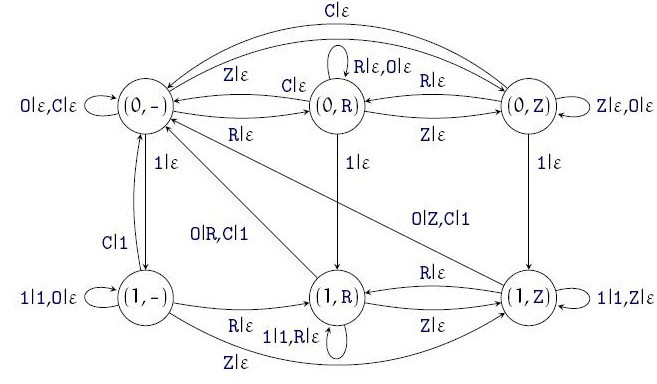
\includegraphics[height=4.2cm]{src/tut10_automat2.jpg}
		\end{figure}
		Was ist...
		\begin{itemize}
	    \item $g^*((0,-), R1O)$\only<1>{?}\only<2->{$= R$}
	    \item $g^{**}((0,-), R1O)$\only<1>{?}\only<3->{$= R$}
	    \item $g^{**}((0,-), R11O)$\only<1>{?}\only<4->{$= 1R$}
		\end{itemize}
\end{frame}

\begin{frame}
	\frametitle{Ihr seid dran...}
 	Entwickelt einen Mealy-Automaten, der...
 	\begin{itemize}
 	  \item nur ein Zustand $z$ hat und $X=Y=\{a,b\}$, $g(z,a)=b$ und $g(z,b)=ba$ erfüllt
 	  \only<1-2>{
    \begin{itemize}
    \item wie sieht $w_1=g^{**}(z,a)$ aus?
    \item $w_2=g^{**}(z,w_1)$, \dots $w_{i+1}=g^{**}(z,w_i)$?
    \item könnte man den Automaten mit weniger Zuständen darstellen?
    \end{itemize}}
     	\only<2>{
        	\begin{center}
		    	\begin{tikzpicture}[shorten >=1pt,node distance=2cm,auto,initial text=]
		    			\node[state,initial] 	(z_0) {$0$};
							\path[->] (z_0) edge [loop above] node [above] {a|b;b|ba} ();

		    	\end{tikzpicture}
		    	\end{center}}

  \item und einen weiteren Automat mit $Z=\mathbb{G}_5$, $X=\{a,b\}$, $Y=\{0,1\}$, bei $b$ gleicher
    Zustand und Ausgabe $0$, bei $a$ einen Zustand weiter und bei jedem
    5.$a$ Ausgabe $1$, sonst Ausgabe $0$. Was tut der Automat?
    		  \only<3>{
    		  \begin{center}
		    	\begin{tikzpicture}[shorten >=1pt,node distance=2cm,auto,initial text=]
		    	\node[state,initial] 	(z_0) {$0$};
		    	\node[state]										(z_1) [right of=z_0]			{$1$};
		    	\node[state]										(z_2) [right of=z_1]			{$2$};
		    	\node[state]										(z_3) [below left of=z_2]	{$3$};
		    	\node[state]										(z_4) [below right of=z_0]{$4$};

					\path[->] (z_0) edge [loop above] node [above] {b|0} ()
													edge							node [above] {a|0} (z_1)
										(z_1) edge [loop above] node [above] {b|0} ()
													edge							node [above] {a|0} (z_2)
										(z_2) edge [loop above] node [above] {b|0} ()
													edge							node [right] {a|0} (z_3)
										(z_3) edge [loop below] node [below] {b|0} ()
													edge							node [below] {a|0} (z_4)
										(z_4) edge [loop below] node [below] {b|0} ()
													edge							node [left]  {a|1} (z_0);
		    	\end{tikzpicture}
		    	\end{center}}
  \end{itemize}
\end{frame}


\begin{frame}
   \frametitle{Der Akzeptor}

   \begin{itemize}
     \item \vspace{-1.4em} Ist der häufigste \textbf{Spezialfall} eines Moore-Automaten
     \item Eine Ausgabe findet nicht bei allen Zuständen statt \pause
     \item Die Zustände $F \subseteq Z$, bei denen eine Ausgabe (immer ein Bit lang) erfolgt, heißen \texttt{akzeptierende Zustände} \\
     Es gilt $F=\{z|h(z)=1\}$ \pause
     \item graphisch werden diese durch Doppelkreise angegeben
     		\begin{center}
        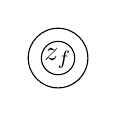
\begin{tikzpicture}
    			\draw(0,0) circle(1.4ex);
      		\node[draw,circle] (qi) at (0,0) {$z_f$};
      	\end{tikzpicture}
      	\end{center} \pause
     \item[]
     \item Ein Wort $w\in X^*$ wird \texttt{akzeptiert}, wenn gilt $f^*(z_0,w)\in F$
     \item Die von einem Akzeptor $A$ \texttt{akzeptierte formale Sprache} ist $L(A)=\{w \in X^* |f^*(z_0,w)\in F\}$
   \end{itemize}
 \end{frame}

 \begin{frame}
 	\frametitle{Ihr seid dran...}
 	Entwickelt einen Akzeptor mit
 	\begin{itemize}
			\item $X=\{a,b\}$, der alle
		    Wörter akzeptiert, bei denen die Anzahl der $a$ durch $5$
		    teilbar ist. (Anzahl der $b$ ist egal).
		    \only<2>{
		    	\begin{center}
		    	\begin{tikzpicture}[shorten >=1pt,node distance=2cm,auto,initial text=]
		    	\node[state,initial,accepting] 	(z_0) {$0$};
		    	\node[state]										(z_1) [right of=z_0]			{$1$};
		    	\node[state]										(z_2) [right of=z_1]			{$2$};
		    	\node[state]										(z_3) [below left of=z_2]	{$3$};
		    	\node[state]										(z_4) [below right of=z_0]{$4$};

					\path[->] (z_0) edge [loop above] node [above] {b} ()
													edge							node [above] {a} (z_1)
										(z_1) edge [loop above] node [above] {b} ()
													edge							node [above] {a} (z_2)
										(z_2) edge [loop above] node [above] {b} ()
													edge							node [right] {a} (z_3)
										(z_3) edge [loop below] node [below] {b} ()
													edge							node [below] {a} (z_4)
										(z_4) edge [loop below] node [below] {b} ()
													edge							node [left]  {a} (z_0);
		    	\end{tikzpicture}
		    	\end{center}}

		  \item $X=\{a,b\}$, der alle
		    Wörter akzeptiert, in denen nirgends hintereinander zwei b
		    vorkommen.
		    \only<3>{
		    	\begin{center}
			  	\begin{tikzpicture}[shorten >=1pt,node distance=2cm,auto,initial text=]
						\node[state,initial,accepting]	(z_0) 								{$0$};
						\node[state,accepting] 					(z_1) [right of=z_0] 	{$1$};
						\node[state] 										(z_2) [right of=z_1] 	{$2$};

						\path[->] (z_0) edge [bend right] node [swap] {b} (z_1)
														edge [loop below] node [swap] {a} ()
											(z_1) edge 							node [swap] {b} (z_2)
														edge [bend right] node [above]{a} (z_0)
											(z_2)	edge [loop below] node [swap] {a,b} ();
					\end{tikzpicture}
					\end{center}}
			\end{itemize}
 \end{frame}

 \begin{frame}
 	\frametitle{Ihr seid dran\ldots}
 	Entwickelt einen Akzeptor\ldots
 	\begin{itemize}
       \item der alle hexadezimalen IP-Adressen der Form $1A.BF.43.0F$ akzeptiert
       \item was ändert sich, wenn man auch Adressen ohne führende $0$
       akzeptieren möchte?
       \item bei Langeweile: versucht alle IP-Adressen bei denen die Blöcke aus
       dezimalen Zahlen zwischen $000$ und $255$ bestehen zu akzeptieren
    \end{itemize}
 \end{frame}

\section{Abschluss}
% Studis anzuregen darüber nachzudenken, ob sie wirklich alles wissen, ansonsten nachlesen oder fragen nachträglich stellen, dann kann in der nächsten Woche nochmal drauf eingegangen werden
\subsection*{}
\begin{frame}
	\frametitle{Zum Schluss...}
	\begin{block}{Was ihr nun wissen solltet!}
	\begin{itemize}
	  	\visible<2->{\item Was ist ein (endlicher) Automat?\\
	  					Aus welchen Teilen besteht er?}
		\visible<3->{\item Worin unterscheiden sich Mealy-, Moore-Automaten und
		endl. Akzeptoren?}
		 \visible<4->{\item Wie sind $f^*,f^{**},g^*,g^{**},h^*,h^{**}$ definiert?}
		 \visible<5->{\item Wie könnte man sie auch noch anders definieren?} \visible<6->{\item Was haben Automaten mit Sprachen zu tun? Warum sind Automaten relevant?}
    \end{itemize}
   	\end{block}

	\visible<7->{
	\begin{block}{Ihr wisst was nicht?}
		Stellt \textbf{jetzt} Fragen!
	\end{block}}
\end{frame}

